\documentclass{beamer}
\usepackage[utf8]{inputenc}
\usepackage[T1]{fontenc}

\usetheme{Cuerna}
\usecolortheme{default}

\title{Progress Report}
\author{Shayan Amani\\}

\date{Jan 2019}
\institute{Department of Computer Science, University of New Hampshire}

\begin{document}

  \begin{frame}
    \titlepage
  \end{frame}


\begin{frame}
    \frametitle{Done}
    
    \begin{itemize}
        \item Laid out a sketch and implemented it to adapt a deep RL method works in offline setting. 
        \item Implemented Value-based Deep RL methods such as:
        \begin{itemize}
            \item Deep Q-Network (DQN) \cite{Mnih2015}
            \item Double DQN \cite{van2016a}
        \end{itemize}
        \item Studied some other proposed alternatives like Dueling Networks\cite{wang2015a}.
        \item Familiarized myself with Open AI's Gym RL frameworks and its popular environments.
    \end{itemize}
\end{frame}

\begin{frame}
    \frametitle{Deep RL Methods Schema}
    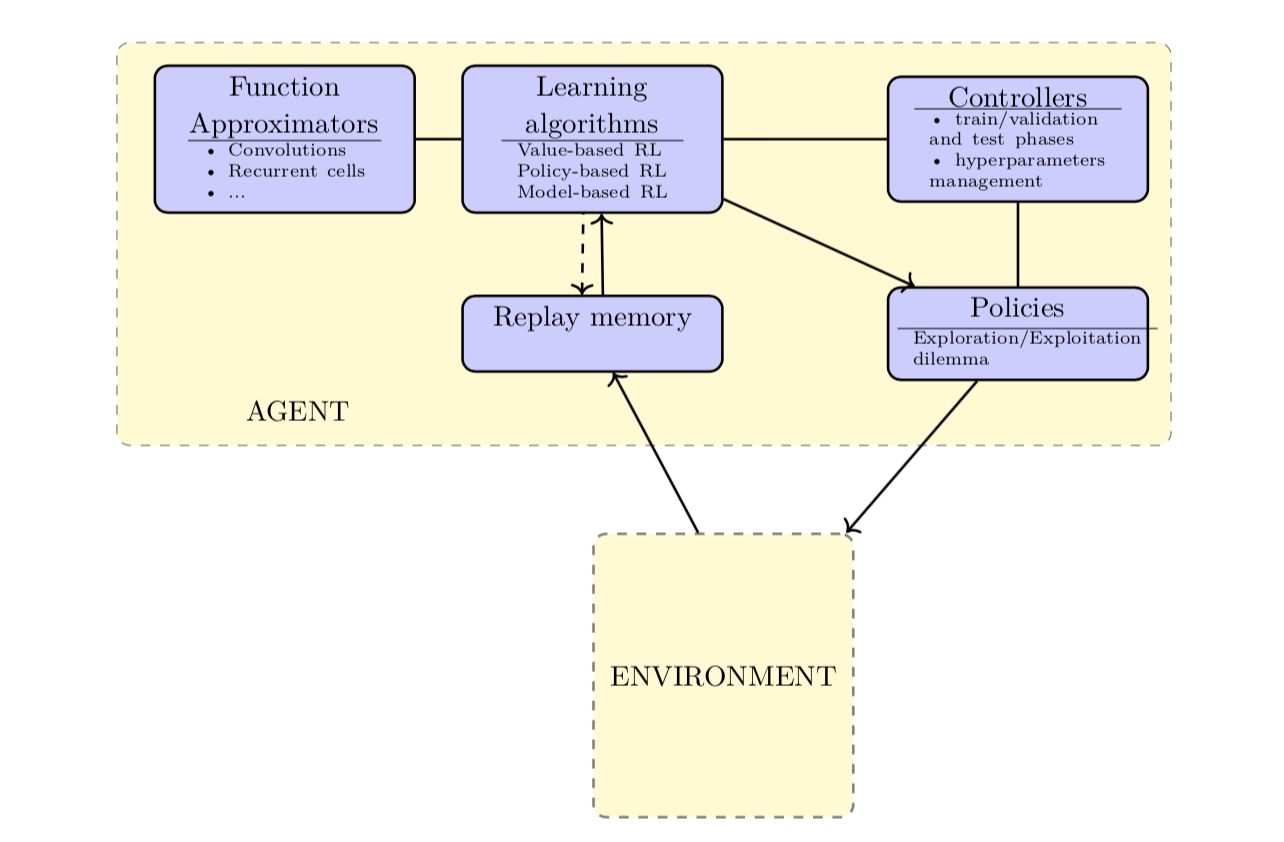
\includegraphics[width=1\columnwidth]{schema_deer.png}    
\end{frame}

\begin{frame}
    \frametitle{DQN Schema}
    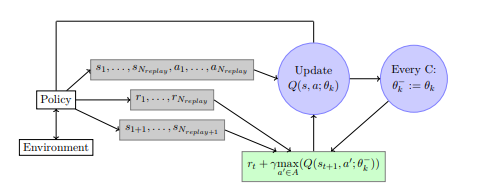
\includegraphics[width=1\columnwidth]{dqn_schema.png}
\end{frame}

\begin{frame}
    \frametitle{To Be Done}
    The following need to be addressed and are proposed here as my future path:
    \begin{itemize}
        \item Random batch sampling from epochs ahead. Inspired by $\epsilon$-greedy approach.
        % \item finding a reliable alternative for $\epsilon$-greedy exploration.
        \item Trying other Loss calculation methods and compare them in practice.
    \end{itemize}
\end{frame}

\bibliographystyle{nips}
\bibliography{lib}

\end{document}